\documentclass[12pt,twoside, lineno]{gsajnl}
% Use the documentclass option 'lineno' to view line numbers
\usepackage{tabularx}
\usepackage{longtable}
\articletype{mp} % article type

\title{Testing pleiotropy vs.\ separate QTL in multiparental populations}

\author[$\ast$,1]{Frederick J. Boehm}
\author[$\dagger$]{Elissa J. Chesler}
\author[$\ast$, $\ddagger$]{Brian S. Yandell}
\author[$\S$]{Karl W. Broman}

\affil[$\ast$]{Department of Statistics, University of Wisconsin-Madison, Madison, Wisconsin 53706}
\affil[$\dagger$]{The Jackson Laboratory, Bar Harbor, Maine 04609}
\affil[$\ddagger$]{Department of Horticulture, University of Wisconsin-Madison, Madison, Wisconsin 53706}
\affil[$\S$]{Department of Biostatistics and Medical Informatics, University of Wisconsin-Madison, Madison, Wisconsin 53706}

\keywords{Quantitative trait locus; pleiotropy; multivariate analysis; linear mixed effects models; systems genetics; ...}

\runningtitle{Testing pleiotropy in MPPs} % For use in the footer
\runningauthor{Boehm \textit{et al.}}




\begin{abstract}

The high mapping resolution of multiparental populations, combined
with technology to measure tens of thousands of phenotypes, presents
an opportunity for quantitative methods to enhance understanding of
the genetic architecture of complex traits. When multiple traits map
to a common genomic region, knowledge of the number of distinct loci
provides important insight into the underlying mechanism and can
assist planning for subsequent experiments. We extend the work of 
\citet{jiang1995multiple} to develop a likelihood ratio test for the case of more than two alleles, for a pair of traits, to test the null hypothesis of pleiotropy against the alternative hypothesis of separate QTL.

We also incorporate polygenic random effects to account for
variation in relatedness among subjects. We use a parametric bootstrap to
determine statistical significance. We apply our methods to a
behavioral genetics data set from Diversity Outbred mice, where we
find evidence for presence of two distinct loci in a 2.5~cM region.
Our methods have been incorporated into the R package
package \texttt{qtl2pleio}.

\end{abstract}
%%%%%%%%%%%%%%%%%%%%%%%%%%%%%%%%%%%%%%%%%%
% Stuff between the two lines of percentage marks may need to be removed before the draft is finalized.
\usepackage[colorinlistoftodos, prependcaption,textsize=tiny]{todonotes}
%% use 'disable' option for todonotes to disable the package, as in the commented line below.
% \usepackage[disable, colorinlistoftodos, prependcaption,textsize=tiny]{todonotes}
\presetkeys%
    {todonotes}%
    {inline,backgroundcolor=yellow}{}

%%%%%%%%%%%%%%%%%%%%%%%%%%%%%%%%%%%%%%%%%%
\setboolean{displaycopyright}{true}

\begin{document}

\maketitle
\thispagestyle{firststyle}
\marginmark
\firstpagefootnote
\correspondingauthoraffiliation{Department of Statistics, 1220 Medical Sciences Center, 1300 University Avenue, Madison, WI 53706. E-mail: frederick.boehm@gmail.com}
\vspace{-11pt}%



Complex trait studies in multiparental populations present new
challenges in statistical methods and data analysis. Among these is
the development of strategies for multivariate trait analysis. The
joint analysis of two or more traits allows one to address additional
questions, such as whether two traits share a single pleiotropic
locus.




Previous research addressed the question of pleiotropy vs.\ separate
QTL in two-parent crosses.
\citet{jiang1995multiple} developed a likelihood
ratio test for pleiotropy vs.\ separate QTL for a pair of traits.
Their approach assumed that each trait was affected by a single QTL.
Under the null hypothesis, the two traits were affected by a common
QTL, and under the alternative hypothesis the two traits were affected
by distinct QTL.
\citet{knott2000multitrait} used linear regression to develop a fast
approximation to the test of \citet{jiang1995multiple}, while
\citet{tian2016dissection} used the methods from
\citet{knott2000multitrait} to dissect QTL hotspots in a F$_2$
population.




Multiparental populations, such
as the Diversity Outbred (DO)mouse population \citep{churchill2012diversity}, enable high-precision
mapping of complex traits \citep{de2014genetics}. The DO
mouse population began with progenitors of the Collaborative
Cross (CC) mice \citep{churchill2004collaborative}
Each DO mouse is a highly heterozygous genetic mosaic
of alleles from the eight CC founder lines. Random
matings among non-siblings have maintained the DO
population for more than 23 generations \citep{chesler2016diversity}.

Several limitations of previous pleiotropy vs.\ separate QTL tests
prevent their direct application in multiparental populations. First,
multiparental populations can have complex patterns of relatedness
among subjects, and failure to account for these patterns of
relatedness may lead to spurious results \citep{yang2014advantages}.
Second, previous tests allowed for only two founder lines
\citep{jiang1995multiple}. Finally, \citet{jiang1995multiple} assumed
that the null distribution of the test statistic follows a chi-square
distribution.

We developed a pleiotropy vs.\ separate QTL test for two traits in
multiparental populations. Our test builds on research that
\citet{jiang1995multiple}, \citet{knott2000multitrait},
\citet{tian2016dissection}, and \citet{zhou2014efficient} initiated.
Our innovations include the accommodation of $k$ founder alleles per
locus (compared to the traditional two founder alleles per locus) and
the incorporation of multivariate polygenic random effects to account
for relatedness. Furthermore, we implemented a parametric bootstrap to
calibrate test statistic values \citep{efron1979,tian2016dissection}.

Below, we describe our likelihood ratio test for pleiotropy vs.\
separate QTL. In simulation studies, we find that it is slightly
conservative, and that it has power to detect two separate loci when
the univariate LOD peaks are strong. We further illustrate our
approach with an application to data on a pair of behavior traits in
a population of 261 DO mice \citep{logan2013high,recla2014precise}.
We find modest evidence for distinct QTL in a 2.5-cM region on mouse
Chromosome 8.


\section{Methods}
\label{sec:materials:methods}

Our strategy involves first identifying two traits that map to a common
genomic region. We then perform a two-dimensional, two-QTL scan over
the genomic region, with each trait affected by one QTL of varying
position. We identify the QTL position that maximizes the likelihood
under pleiotropy (that is, along the diagonal where the two QTL are at
a common location), and the ordered pair of positions that maximizes
the likelihood under the model where the two QTL are allowed to be
distinct. The logarithm of the ratio of the two likelihoods is our
test statistic. We calibrate this test statistic with a parametric
bootstrap.

\subsection{Data structures}

The data consist of three objects. The first is an $n$ by $k$ by $m$
array of allele probabilities for $n$ subjects with $k$ alleles and
$m$ marker positions on a single chromosome [derived from the observed
SNP genotype data by a hidden Markov model; see
\citet{broman2019rqtl2}]. The second object is an $n$ by 2 matrix of
phenotype values. Each column is a phenotype and each row is a
subject. The third object is an $n$ by $c$ matrix of covariates, where
each row is a subject and each column is a covariate.

One additional object is the genotype-derived kinship matrix, which is
used in the linear mixed model to account for population structure. We
are focusing on a defined genomic interval, and we prefer to use a
kinship matrix derived by the ``leave one chromosome out'' (LOCO)
method \citep{yang2014advantages}, in which the kinship matrix is
derived from the genotypes for all chromosomes except the chromosome
under test.




\subsection{Statistical Models}

Focusing on a pair of traits and a particular genomic region of
interest, the next step is a two-dimensional, two-QTL
scan \citep{jiang1995multiple}. We consider two QTL with each
affecting a different trait, and consider all possible pairs of
locations for the two QTL. For each pair of positions, we fit
the multivariate linear mixed effects model defined in Equation
\ref{eqn:model1}. Note that we have
assumed an additive genetic model throughout our analyses, but
extensions to design matrices that include dominance are
straightforward.


\begin{equation}
vec(Y) = X vec(B) + vec(G) + vec(E)
\label{eqn:model1}
\end{equation}
where $Y$ is the $n$ by $2$ matrix of phenotypes values;
$X$ is a $2n$ by $2(k + c)$
matrix that contains the $k$ allele probabilities for the two QTL
positions and the $c$
covariates in diagonal blocks; $B$ is a $(k + c)$ by $2$ matrix of
allele effects and covariate effects; $G$ is a $n$ by $2$ matrix of
random effects; and $E$ is a $n$ by $2$ matrix of random errors. $n$
is the number of mice. The `vec' operator stacks columns from a matrix
into a single vector. For example, a 2 by 2 matrix inputted to `vec'
results in a vector with length 4. Its first two entries are the
matrix's first column, while the third and fourth entries are the
matrix's second column.


We also impose distributional assumptions on $G$ and $E$:

\begin{equation}
G \sim MN_{n x 2}(0, K, V_g)
\label{eqn:model2}
\end{equation}

and

\begin{equation}
E \sim MN_{nx2}(0, I, V_e)
\label{eqn:model3}
\end{equation}
where $MN_{n x 2}(0, V_r, V_c)$ denotes the matrix-variate ($n$ by 2)
normal distribution with mean being the $n$ by $2$ matrix with all
zero entries and row covariance $V_r$ and column covariance $V_c$. We
assume that $G$ and $E$ are independent.


\subsection{Parameter inference and log likelihood calculation}

Inference for parameters in multivariate linear mixed effects models
is notoriously difficult and can be computationally intense
\citep{meyer1989restricted,meyer1991estimating}. Thus, we estimate
$V_g$ and $V_e$ under the null hypothesis of no QTL, and then take
them as fixed and known in our two-dimensional, two-QTL genome scan.
We use restricted maximum likelihood methods to fit the
model:

\begin{equation}
vec(Y) = X_0vec(B) + vec(G) + vec(E)
\label{model}
\end{equation}
where $X_0$ is a $2n$ by $2(c + 1)$ matrix whose first column of each
diagonal block in $X_0$ has all entries equal to one (for an intercept); the remaining
columns are the covariates.

We draw on our R implementation \citep{gemma2} of the
GEMMA algorithm for fitting a multivariate linear mixed effects model
with expectation-maximization \citep{zhou2014efficient}. We use
restricted maximum likelihood fits for the variance components $V_g$
and $V_e$ in subsequent calculations of the generalized least squares
solution $\hat B$.

\begin{equation}
    \hat B = (X^T\hat\Sigma^{-1}X)^{-1}X^T\hat\Sigma^{-1}vec(Y)
\end{equation}

\noindent where

\begin{equation}
    \hat\Sigma = \hat V_g \otimes K + \hat V_e \otimes I_n
    \label{cov}
\end{equation}

\noindent where $\otimes$ denotes the Kronecker product, $K$ is the
kinship matrix, and $I_n$ is a n by n
identity matrix. We then calculate the log likelihood for a normal
distribution with mean $X vec(\hat B)$ and covariance $\hat \Sigma$
that depends on our estimates of $V_g$ and $V_e$ (Equation \ref{cov}).

\subsection{Pleiotropy vs.\ separate QTL hypothesis testing framework}

Our test applies to two traits considered simultaneously. Below,
$\lambda_1$ and $\lambda_2$ denote putative locus positions for traits
one and two. We quantitatively state the competing hypotheses for our
test as:

\begin{eqnarray}
H_0: \lambda_1 = \lambda_2 \nonumber\\
H_A: \lambda_1 \neq \lambda_2
\label{eqn:hypotheses}
\end{eqnarray}

\noindent Our likelihood ratio test statistic is:

\begin{equation}
\text{LOD} = \log_{10} \left[ \frac{\max_{\lambda_1, \lambda_2} L(B, \Sigma, \lambda_1, \lambda_2)}{
    \max_\lambda L(B, \Sigma, \lambda, \lambda)} \right]
\label{eqn:test-statistic}
\end{equation}
where $L$ is the likelihood for fixed QTL positions,
maximized over all other parameters.

\subsection{Visualizing profile LOD traces}

The output of the above analysis is a two-dimensional log$_{10}$ likelihood
surface. To visualize these results, we followed an innovation of \citet{zeng2000genetic} and
\citet{tian2016dissection}, and plot three traces: the results along the
diagonal (corresponding to the null hypothesis of pleiotropy), and
then the profiles derived by fixing one QTL's position
and maximizing over the other QTL's position.

We define the LOD score for our test:

\begin{equation}
\text{LOD}(\lambda_1, \lambda_2) = ll_{10}(\lambda_1, \lambda_2) - \max ll_{10}(\lambda, \lambda)
\label{eq:lodpvl}
\end{equation}
where $ll_{10}$ denotes log$_{10}$ likelihood.

We follow \citet{zeng2000genetic} and \citet{tian2016dissection} in
defining profile LOD by the equation

\begin{equation}
\text{profile LOD}_1(\lambda_1) = \max_{\lambda_2}\text{LOD}(\lambda_1, \lambda_2)
\label{eq:profilelod}
\end{equation}
We define profile LOD$_2(\lambda_2)$ analogously.
The maximum value for the profile LOD$_1$
profile LOD$_2$ traces are the same and are non-negative, and give the
overall LOD test statistic.

We construct the pleiotropy trace by calculating the log-likelihoods
for the pleiotropic models at every position.

\begin{equation}
LOD_{p}(\lambda) = ll_{10}(\lambda, \lambda) - \max ll_{10}(\lambda, \lambda)
\label{eq:lodp}
\end{equation}
By definition, the maximum value for this pleiotropy trace
is zero.






\subsection{Bootstrap for test statistic calibration}

We use a parametric bootstrap to calibrate our test statistic
\citep{efron1979}. While \citet{jiang1995multiple} used quantiles of a
chi-squared distribution to determine p-values, this does not account
for the two-dimensional search over QTL positions.
We follow the approach of \citet{tian2016dissection}, and identify
the maximum likelihood estimate of the QTL position under the null
hypothesis of pleiotropy.
We then use the inferred model parameters under that model and with
the QTL at that position to simulate bootstrap data sets according to
the model in equations \ref{eqn:model1}--\ref{eqn:model3}.
For each of $b$ bootstrap data sets, we
perform a two-dimensional QTL scan (over the genomic region of
interest) and derive the test
statistic value. We treat these $b$ test statistics as the
empirical null distribution, and calculate a p-value as the
proportion of the $b$ bootstrap test statistics that equal or exceed
the observed one, with the original data,
$p = \# \{ i:\text{LOD}^*_i \geq \text{LOD}\} / b$
where $\text{LOD}_i^*$ denotes the LOD score for the $i$th bootstrap
replicate and LOD is the observed test statistic.



\subsection{Data \& Software Availability}

Our methods have been implemented in an R package, \texttt{qtl2pleio},
available at GitHub:

\href{https://github.com/fboehm/qtl2pleio}{https://github.com/fboehm/qtl2pleio}

\noindent Custom R code for our analyses and simulations are at GitHub:

\href{https://github.com/fboehm/qtl2pleio-manuscript}{https://github.com/fboehm/qt2pleio-manuscript}

\noindent The data from \citet{recla2014precise} and
\citet{logan2013high} are available at the Mouse Phenome Database:

\href{https://phenome.jax.org/projects/Chesler4}{https://phenome.jax.org/projects/Chesler4} and \href{https://phenome.jax.org/projects/Recla1}{https://phenome.jax.org/projects/Recla1}.

\noindent They are also available in R/qtl2 format at
\href{https://github.com/rqtl/qtl2data}{https://github.com/rqtl/qtl2data}.




\section{Simulation studies}

We performed two types of simulation studies, one for type I error
rate assessment and one to characterize the power to detect separate
QTL. To simulate traits, we specified $X$, $B$, $V_g$, $K$, and $V_e$
matrices (Equations \ref{eqn:model1}--\ref{eqn:model3}). For both we
used the allele probabilities from a single genomic region derived
empirically from data for a set of 479 Diversity Outbred mice from
\citet{keller2018}.

\subsection{Type I error rate analysis}

To quantify type I error rate ({\em i.e.}, false positive rate), we
simulated 400 pairs of traits for each of eight sets of parameter
inputs (Table~\ref{table-typeI}). We used a $2^3$ factorial
experimental design with three factors: allele effects difference,
allele effects partitioning, and genetic correlation, \textit{i.e.},
the off-diagonal entry in the 2 by 2 matrix $V_g$.

\begin{table}
\begin{center}
  \caption{Type I error rates for all runs in our $2^3$
    experimental design. We set (marginal) genetic variances
    (\emph{i.e.}, diagonal elements of $V_g$) to 1 in all runs. $V_e$
    was set to the 2 by 2 identity matrix in all runs. We used allele
    probabilities at a single genetic marker to simulate traits for
    all eight sets of parameter inputs. In the
    column ``Allele effects partitioning'', ``ABCD:EFGH'' means that lines
    A--D carry one QTL allele while lines E--H carry the other allele.
    ``F:ABCDEGH'' means the QTL has a private allele in strain F.}
  \label{table-typeI}

  \bigskip

\small
  \begin{tabular}{ c | c | c | c | c}
    \hline
    Run & $\Delta$(Allele effects) & Allele effects partitioning & Genetic correlation & Type I error rate \\ \hline
    1 & 6 & ABCD:EFGH & 0 & 0.032\\
    2 & 6 & ABCD:EFGH & 0.6 & 0.035\\
    3 & 6 & F:ABCDEGH & 0 & 0.040\\
    4 & 6 & F:ABCDEGH & 0.6 & 0.045\\
    5 & 12 & ABCD:EFGH & 0 & 0.038\\
    6 & 12 & ABCD:EFGH & 0.6 & 0.042\\
    7 & 12 & F:ABCDEGH & 0 & 0.025\\
    8 & 12 & F:ABCDEGH & 0.6 & 0.025\\
    \hline
  \end{tabular}
\end{center}
  \end{table}

We chose two strong allele effects difference values, 6 and 12. These
ensured that the univariate phenotypes mapped with high LOD scores to
the region of interest. For the allele partitioning factor, we used
either equally frequent QTL alleles, or a private allele in the CAST
strain (F). For the residual genetic correlation (the off-diagonal
entry in $V_g$), we considered the values 0 and 0.6. The marginal
genetic variances (\textit{i.e.}, the diagonal entries in $V_g$) for
each trait were always set to one.

We performed 400 simulation replicates per set of parameter inputs,
and each used $b = 400$ bootstrap samples. For each bootstrap sample, we calculated the
test statistic (Equation \ref{eqn:test-statistic}). We then compared
the test statistic from the simulated trait against the empirical
distribution of its 400 bootstrap test statistics. When the simulated
trait's test statistic exceeded the 0.95 quantile of the empirical
distribution of bootstrap test statistics, we rejected the null
hypothesis. We observed that the test is slightly conservative over
our range of parameter selections (Table~\ref{table-typeI}), with
estimated type I error rates $<$ 0.05.


\subsection{Power analysis}

We also investigated the power to detect the presence of two
distinct QTL. We used a 2 $\times$ 2 $\times$ 5 experimental design, where our
three factors were allele effects difference, allele effects
partitioning, and inter-locus distance. The two levels of allele
effects difference were 1 and 2. The two levels of allele effects
partitioning were as in the type I error rate studies, ABCD:EFGH and
F:ABCDEGH (Table~\ref{table-letters}). The five levels of interlocus
distance were 0, 0.5, 1, 2, and 3 cM. $V_g$ and $V_e$ were both set to
the 2 by 2 identity matrix in all power study simulations.

We simulated 400 pairs of traits per set of parameter inputs. For
each simulation replicate, we calculated the likelihood ratio test
statistic. We then applied our parametric bootstrap to calibrate the
test statistics. For each simulation replicate, we used $b = 400$ bootstrap
samples. Because the bootstrap test statistics within a single set of
parameter inputs followed approximately the same distribution, we
pooled the $400 * 400 = 160,000$ bootstrap samples per set of
parameter inputs and compared each test statistic to the empirical
distribution derived from the 160,000 bootstrap samples. However, for
parameter inputs with interlocus distance equal to zero, we didn't
pool the 160,000 bootstrap samples; instead, we proceeded by
calculating power (\textit{i.e.}, type I error rate, in this case), as we did in the
type I error rate study above.

\begin{figure}
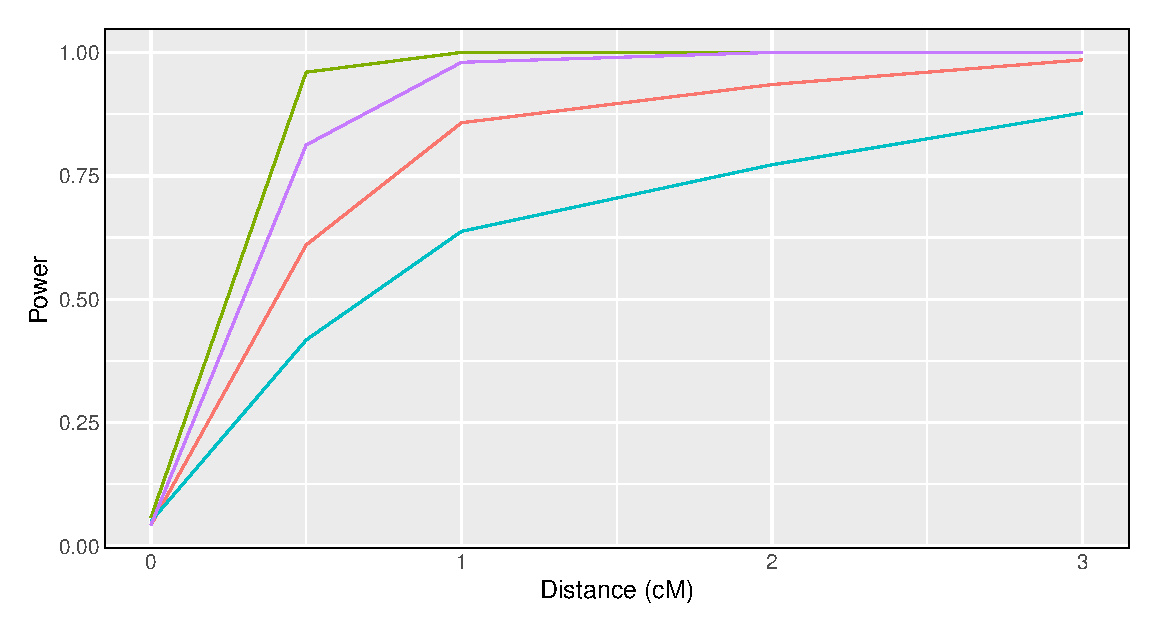
\includegraphics[width = \textwidth]{../R/power-curves.eps}
\caption{Pleiotropy vs.\ separate QTL power curves for each of four
  sets of parameter settings. Factors that differ among the four
  curves are allele effects difference and allele partitioning. Red denotes high allele effects difference, while black is the low allele effects difference. Solid line denotes the even allele partitioning (ABCD:EFGH), while dashed line denotes the uneven allele partitioning (F:ABCDEGH).}
\label{fig:power}
\end{figure}

We present our power study results in Figure~\ref{fig:power}.
Power increases as interlocus distance increases. The top two curves
correspond to the case where the QTL effects are largest. For each value
for the QTL effect, power is greater when the QTL alleles are equally
frequent, and smaller when a QTL allele is private to one strain. One
can have high power to detect that the two traits have distinct QTL
when they are separated by $>$ 1~cM and when the QTL have large effect.


\section{Application}
\label{sec:app}

To illustrate our methods, we applied our test to data from
\citet{logan2013high} and \citet{recla2014precise}, on 261 DO mice
measured for a set of behavioral phenotypes.
\citet{recla2014precise} identified \textit{Hydin} as the gene that
underlies a QTL on Chromosome 8 at 57 cM for the ``hot plate latency''
phenotype (a measure of pain tolerance). The phenotype ``percent time in light''
in a light-dark box (a measure of anxiety) was
measured on the same set of mice \citep{logan2013high} and also shows a QTL near
this location, which led us to ask whether the same locus affects both traits.
The two traits show a correlation of $-0.15$ (Figure~\ref{fig:scatter}).

QTL analysis with the LOCO method, and using sex as an additive
covariate, showed multiple suggestive QTL for each
phenotype (Figure~\ref{fig:genomewide10-22}; Table~\ref{table-peaks}). For our investigation of
pleiotropy, we focused on the interval 53--64~cM on Chromosome 8.
The univariate QTL results for this region are shown in
Figure~\ref{fig:chr8-lod}.

\begin{figure}
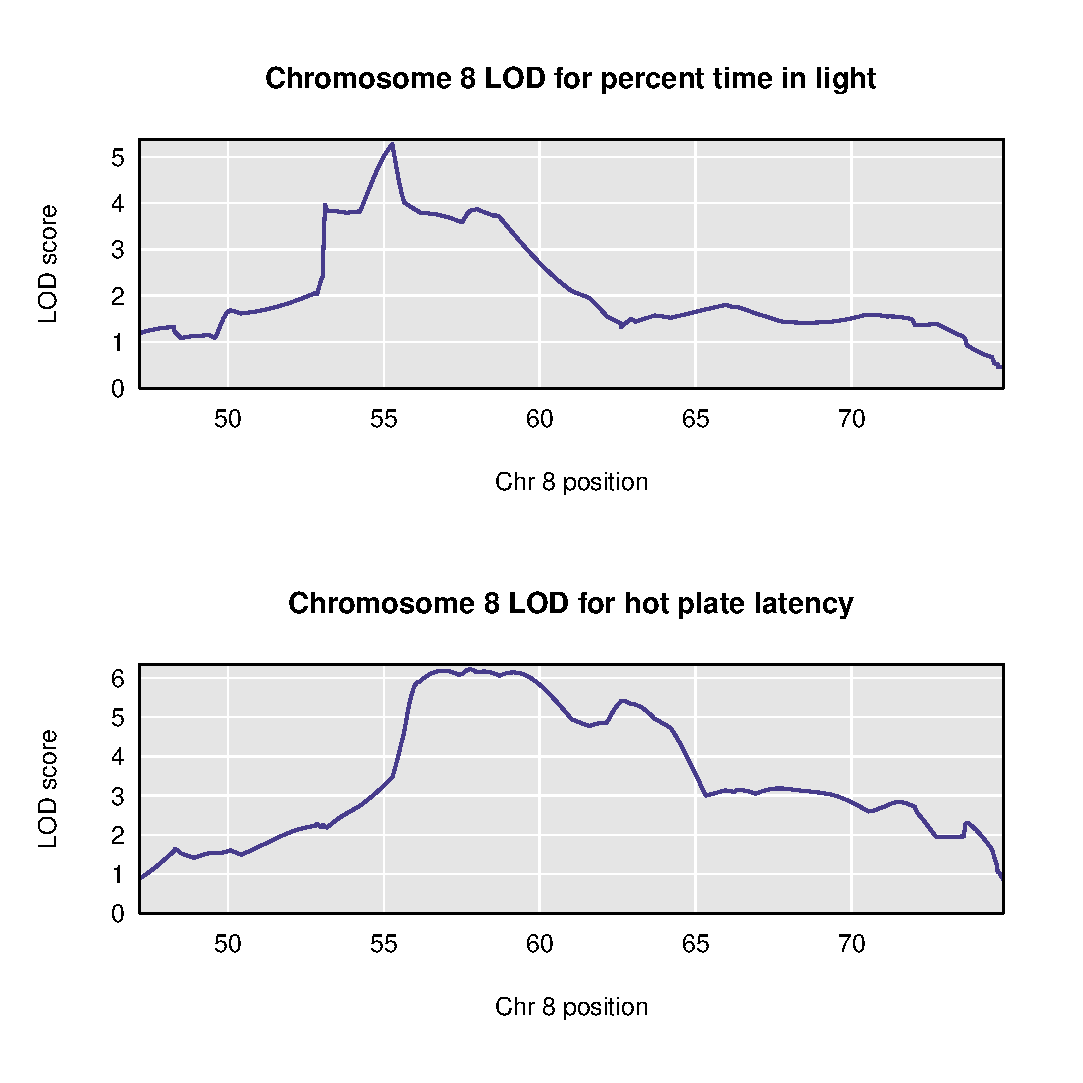
\includegraphics[width = \textwidth]{../Rmd/chr8-lods.eps}
\caption{Chromosome 8 univariate LOD scores for percent time in light
  and hot plate latency reveal broad, overlapping peaks between 53 cM
  and 64 cM. The peak for percent time in light spans the region from
  approximately 53 cM to 60 cM, with a maximum near 55 cM. The peak
  for hot plate latency begins near 56 cM and ends about 64 cM.}
\label{fig:chr8-lod}
\end{figure}


The estimated QTL allele effects for the two traits are quite
different (Figure~\ref{fig:chr8-effects}).
With the QTL placed at 55~cM, for ``percent time in light'', the WSB and PWK alleles are associated
with large phenotypes and NOD with low phenotypes.
For ``hot plate latency'', on the other hand,
CAST and NZO show low phenotypes and NOD and PWK are near the center.

\begin{figure}
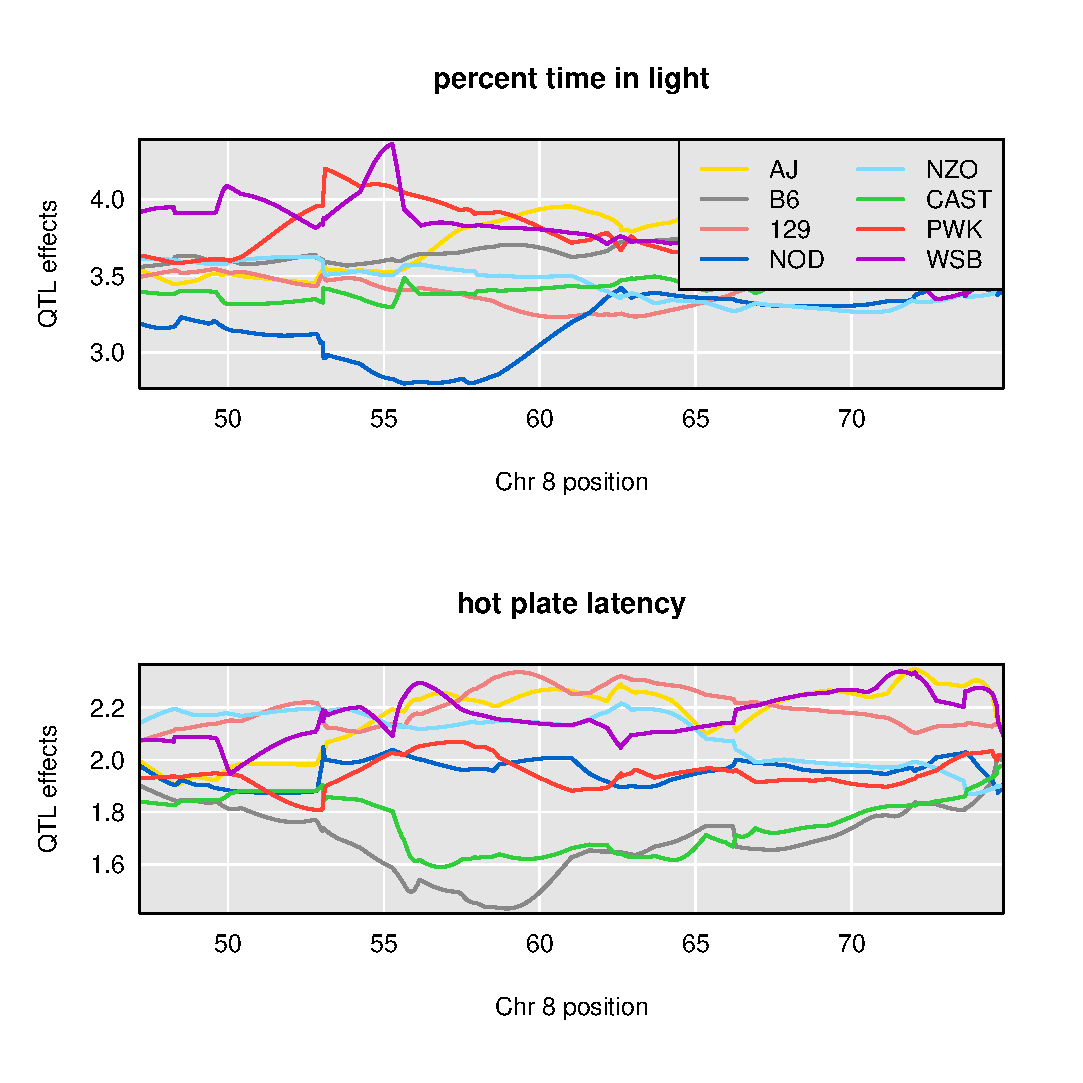
\includegraphics[width = \textwidth]{../Rmd/coefs.eps}
\caption{Chromosome 8 univariate LOD scores for percent time in light
  and hot plate latency reveal broad, overlapping peaks between 53 cM
  and 64 cM. The peak for percent time in light spans the region from
  approximately 53 cM to 60 cM, with a maximum near 55 cM. The peak
  for hot plate latency begins near 56 cM and ends about 64 cM.}
\label{fig:chr8-effects}
\end{figure}

In applying our test for pleiotropy,  we performed a two-dimensional, two-QTL scan for the pair of
phenotypes. With these results, we created a profile LOD plot
(Figure~\ref{fig:profiles}). The profile LOD for ``percent
time in light'' (in brown) peaks near 55 cM, as was seen in the univariate
analysis.  The profile LOD for ``hot plate latency'' (in blue) peaks near 57 cM,
also similar to the univariate analysis.
The pleiotropy trace (in gray) peaks near 55 cM.

\begin{figure}
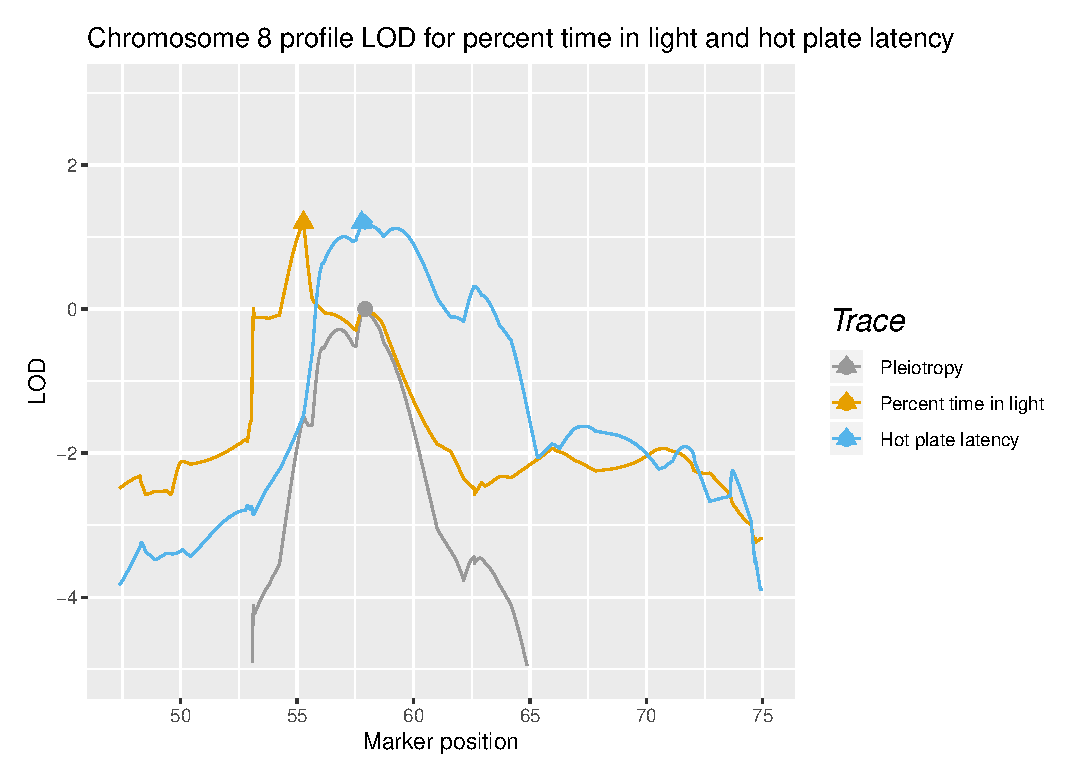
\includegraphics[width = \textwidth]{../Rmd/profile.eps}
\caption{Profile LOD curves for the pleiotropy vs.\ separate QTL
  hypothesis test for ``percent time in light'' and ``hot plate latency''.
  Gray trace denotes pleiotropy LOD values. Triangles denote the
  univariate LOD maxima, while diamonds denote the profile LOD maxima.
  For ``percent time in light'', the brown triangle obscures the
  smaller brown diamond. Likelihood ratio test statistic value
  corresponds to the height of the blue and brown traces at their
  maxima.}
\label{fig:profiles}
\end{figure}

The likelihood ratio test statistic for the test of pleiotropy was
1.2. Based on a parametric bootstrap with 1,000 bootstrap replicates,
the estimated p-value was 0.11, indicating weak
evidence for distinct QTL for the two traits.









\section{Discussion}

We developed a test of pleiotropy vs.\ separate QTL for multiparental
populations, extending the work of \citet{jiang1995multiple} for
multiple alleles and with a linear mixed model to account for
population structure \citep{kang2010variance, yang2014advantages}. Our simulation
studies indicate that the test has power to detect presence of
separate loci, especially when univariate trait associations are
strong (Figure~\ref{fig:power}). Type I error rates indicate that our
test is slightly conservative (Table~\ref{table-typeI}).

In the application of our method to two behavioral phenotypes in a
study of 261 Diversity Outbred mice
\citep{recla2014precise,logan2013high}, we obtained weak evidence
(p=0.11) for the presence of two distinct QTL, with one QTL (which
contained the \textit{Hydin} gene) affecting only ``hot plate latency'' and a
second QTL affecting ``percent time in light'' (Figure~\ref{fig:profiles}).

Founder allele effects plots provide further evidence for the presence
of two distinct loci. As \citet{macdonald2007joint} and
\citet{king2012genetic} have demonstrated in their analyses of multiparental
\emph{Drosophila} populations, a biallelic pleiotropic QTL would result in
allele effects plots that have similar patterns. While we don't know
that ``percent time in light'' and ``hot plate latency'' arise from
biallelic QTL, the dramatic differences that we observe in allele
effects patterns further support the argument for two distinct loci.

We have implemented our methods in an R package
\texttt{qtl2pleio}, but analyses can be computationally intensive and
time consuming. \texttt{qtl2pleio} is written mostly in R, and so we
could likely obtain improved computational speed by porting parts of
the calculations to a compiled langugage such as C or C++.
To accelerate our multi-dimensional QTL
scans, we have integrated C++ code into \texttt{qtl2pleio},
using the Rcpp package \citep{eddelbuettel2011rcpp}.

Another computational bottleneck is the estimation of the variance
components $V_g$ and $V_e$. In future research, we hope to extend our
work for the joint analysis of more than two traits, and we will
consider other strategies for variance component estimation, including
that described by \citet{hannah2018limmbo}, who implement a bootstrap
strategy to estimate variance components for lower-dimensional
phenotypes before combining bootstrap variance component estimates
into valid covariance matrices for the full multivariate phenotype.


We view tests of pleiotropy as complementary to 
mediation tests and related methods that have become popular for
inferring biomolecular causal relationships
\citep{chick2016defining,schadt2005integrative,baron1986moderator}. A
mediation test proceeds by including a putative mediator as a
covariate in the regression analysis of phenotype and QTL genotype;
a substantial reduction in the association between
genotype and phenotype corresponds to evidence of mediation. 


Mediation analyses and our pleiotropy test ask distinct, but related, questions. Mediation analysis seeks to establish causal relationships among traits, including molecular traits, or dependent biological and behavioral processes. Pleiotropy tests examine whether two traits share a single source of genetic variation, which may act in parallel or in a causal network. Pleiotropy is required for causal relations among traits. In many cases, the pleiotropy hypothesis is the only reasonable one. 

\citet{schadt2005integrative} argued that
both pleiotropy tests and causal inference methods may contribute to gene network
reconstruction. They developed a model selection strategy, based on
the Akaike Information Criterion \citep{akaike1974new}, to determine which
causal model is most compatible with the observed data.
\citet{schadt2005integrative} extended the methods of
\citet{jiang1995multiple} to consider more complicated alternative
hypotheses, such as the possibility of two QTL, one of which
associates with both traits, and one of which associates with only one
trait. As envisioned by \citet{schadt2005integrative}, we foresee
complementary roles emerging for our pleiotropy test
and mediation tests in the dissection of complex trait genetic
architecture.

CAPE (Combinatorial Analysis of Pleiotropy and Epistasis) is a strategy for identifying higher-order relationships among traits and marker genotypes \citep{tyler2013cape}. \citet{tyler2017epistatic} used CAPE to identify epistatic gene networks in Diversity Outbred mice. \citet{tyler2016} found evidence for weak epistasis in a large intercross population. 

CAPE uses univariate linear models that are distinct from those in our pleiotropy test. A CAPE starts with founder allele probabilities at all markers and a collection of two or more traits \citep{tyler2017epistatic}. After eigendecomposition to get two or more eigentraits, univariate QTL scans are performed and founder allele effects are estimated at all markers (or a subset of all markers). Next, you identify markers with sufficiently strong effects of at least one founder allele. The \texttt{cape} R package provides options to examine only those markers that have little pairwise linkage disequilibrium. Resulting eigentrait - marker - founder allele triples are then subjected to a second model fitting. This second round of modeling involves two eigentrait - marker - founder allele triples that share an eigentrait. The shared (univariate) eigentrait is modeled as a linear function of the two founder allele dosages and their interaction. 

In comparing CAPE and our pleiotropy test, it's important to recognize that the two methods ask fundamentally different questions. CAPE enables assessment of interactions among specific founder allele dosages at two (possibly identical) markers while examining one eigentrait at a time. Our pleiotropy test, on the other hand, jointly models two phenotypes and quantifies the evidence against the pleiotropy hypothesis by performing a two-dimensional QTL scan over a genomic region. Our multivariate linear models accommodate interactions between founder allele dosages at two markers, but we haven't yet incorporated this functionality into our software. It is one direction for future research.

Technological advances
in mass spectrometry and RNA sequencing have enabled the acquisition of
high-dimensional biomolecular phenotypes
\citep{ozsolak2011rna,han2012multi}. Multiparental populations in
\textit{Arabidopsis}, maize, wheat, oil palm, rice,
\textit{Drosophila}, yeast, and other organisms enable high-precision
QTL mapping \citep{yu2008genetic, tisne2017identification,
  stanley2017genetic, raghavan2017approaches, mackay2012drosophila,
  kover2009multiparent, cubillos2013high}. The need to analyze
high-dimensional phenotypes in multiparental populations compels the
scientific community to develop tools to study genotype-phenotype
relationships and complex trait architecture. Our test, and its future
extensions, will contribute to these ongoing efforts.




\subsection*{Acknowledgments}

The authors thank Lindsay Traeger, Julia Kemis, and Rene Welch for
valuable suggestions to improve the manuscript. This work was
supported in part by National Institutes of Health grant R01GM070683
(to K.W.B.). The research made use of compute resources and assistance
of the UW-Madison Center For High Throughput Computing (CHTC) in the
Department of Computer Sciences at UW-Madison, which is supported by
the Advanced Computing Initiative, the Wisconsin Alumni Research
Foundation, the Wisconsin Institutes for Discovery, and the National
Science Foundation, and is an active member of the Open Science Grid,
which is supported by the National Science Foundation and the U.S.
Department of Energy's Office of Science.





\bibliography{research,qtl2pleio-manuscript}

\newpage
\appendix

% supplemental tables
\renewcommand{\thetable}{\textbf{S\arabic{table}}}
\setcounter{table}{0}


\begin{table}
  \caption{Eight founder lines and their one-letter abbreviations.}
  \label{table-letters}
\begin{center}
\small
  \begin{tabular}{ c | c }
    \hline
    Founder allele & One-letter abbreviation \\ \hline
    A/J & A \\
    C57BL/6J & B \\
    129S1/SvImJ & C \\
    NOD/ShiLtJ & D\\
    NZO/H1LTJ & E\\
    Cast/EiJ & F\\
    PWK/PhJ & G\\
    WSB/EiJ & H\\
    \hline
  \end{tabular}

\end{center}
  \end{table}

\clearpage

  % latex table generated in R 3.5.1 by xtable 1.8-3 package
% Tue Nov 20 10:28:47 2018
\begin{table}
\caption{Both ``hot plate latency'' and ``percent time in light''
  demonstrate multiple QTL peaks with LOD scores above 5.}
  \label{table-peaks}
\begin{center}
\begin{tabular}{l|lrr}
  \hline
phenotype & chr & pos & LOD score \\
   \hline
percent time in light & 8 & 55.28 & 5.27 \\
 hot plate latency & 8 & 57.77 & 6.22 \\
 percent time in light & 9 & 36.70 & 5.42 \\
 hot plate latency & 9 & 46.85 & 5.22 \\
 percent time in light & 11 & 63.39 & 6.46 \\
 hot plate latency & 12 & 43.52 & 5.13 \\
 percent time in light & 15 & 15.24 & 5.67 \\
 hot plate latency & 19 & 47.80 & 5.48 \\
   \hline
\end{tabular}
\end{center}
\end{table}







\clearpage


% supplemental figures
\renewcommand{\thefigure}{\textbf{S\arabic{figure}}}
\setcounter{figure}{0}

\begin{figure}
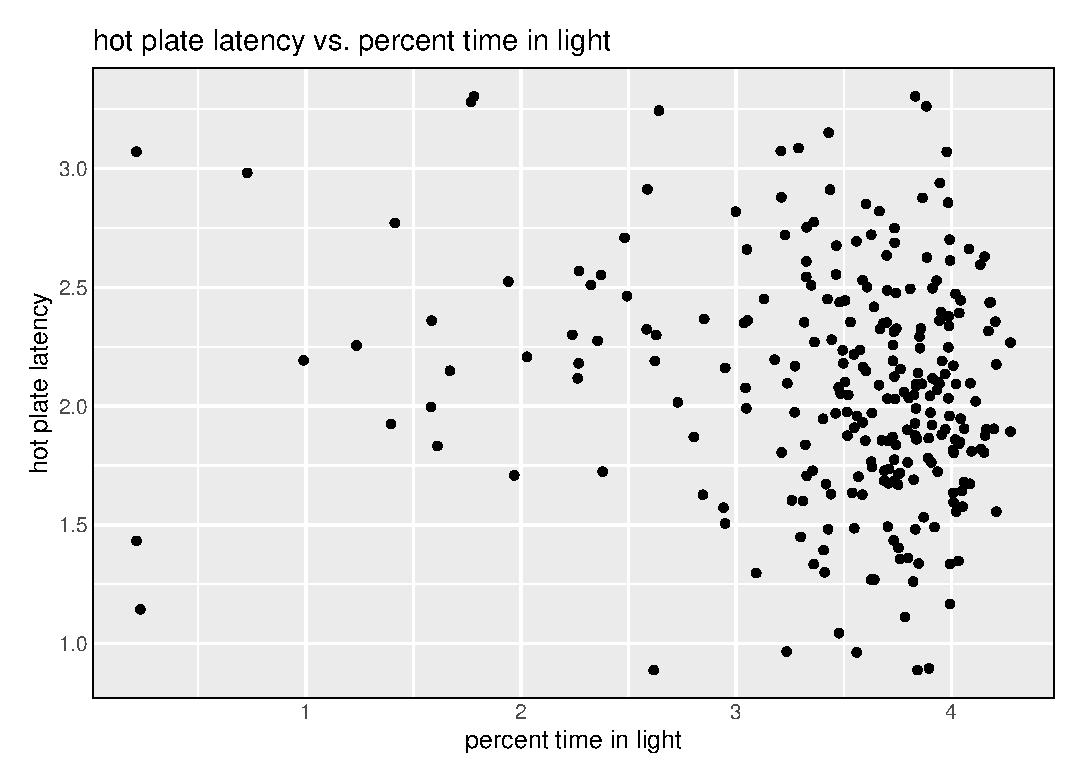
\includegraphics[width = \textwidth]{../Rmd/scatter.eps}
\caption{Scatter plot of ``hot plate latency'' against ``percent time in
  light'', after applying logarithm transformations and winsorizing
  both traits.}
\label{fig:scatter}
\end{figure}


\begin{figure}
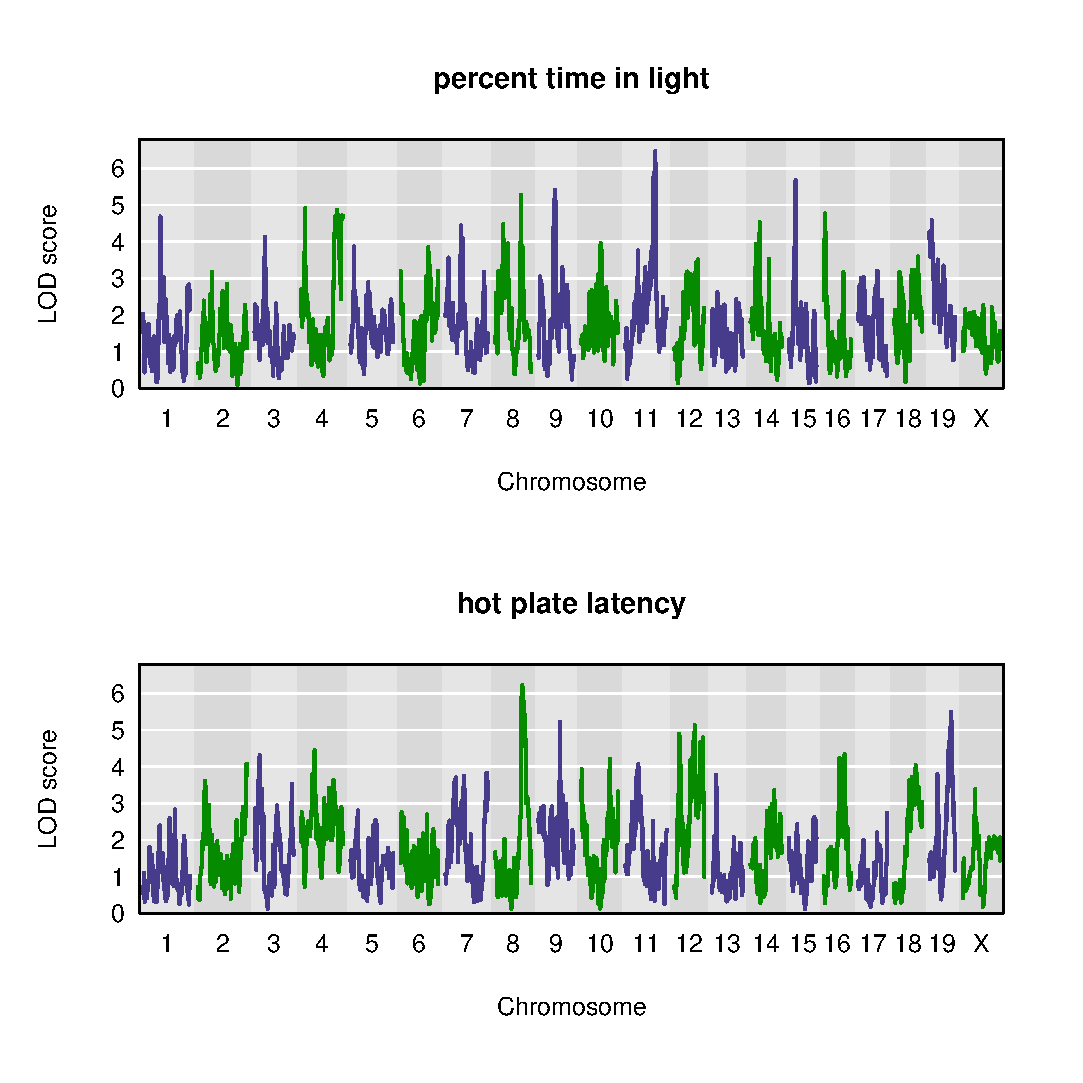
\includegraphics{../Rmd/genomewide_lods_10-22.eps}
\caption{Genome-wide QTL scan for percent time in light reveals
  multiple QTL, including one on Chromosome 8.}
\label{fig:genomewide10-22}
\end{figure}








\end{document}
